\section{System Design and UI Elements}

\subsection{System Architectures}

    \begin{figure}[htp]
    \centering
    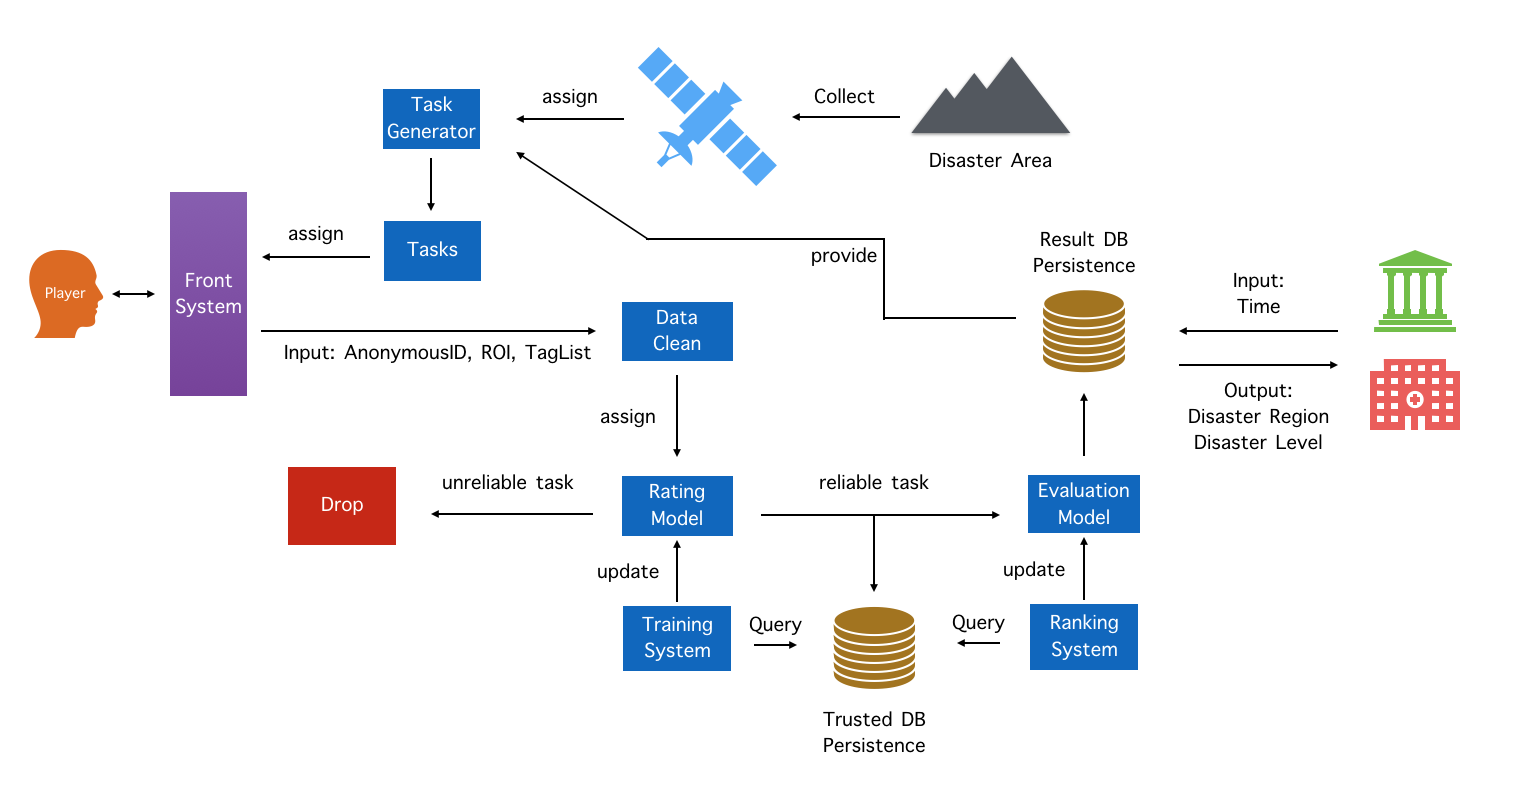
\includegraphics[width=\textwidth]{figures/system}
    \caption{System Design Overview}
    \label{fig:roiweight}
    \end{figure}

\subsection{Algorithm for Data Aggregation}
\subsection{Technologies used for implementation}

  For a prototype, we decided to use the following framework to implement everthing:

  \begin{itemize}
    \item Polymer
    \item Node.js
    \item MongoDB
  \end{itemize}
  \subsection{Front End}
  \subsection{Back End}
  
\subsection{User Interfaces of the system}
\subsection{Summary}

    \begin{itemize}
      \item Task Generator combines trusted results assign to players;
      \item Always treat player as new player, but integrated as old player if exists;
      \item Use ROI matching rate as graph edge weight, eigenvalue as trust value of player;
      \item Disaster Evaluation use pre-defined weight, then defined the disaster level
    \end{itemize}
